\subsection{Switch vs. Hub}
\label{sec:geswitchtes_netz}

Zu Beginn sei erst einmal beschrieben, wie ein Hub und ein Switch funktionieren, denn dies ist relevant für die Betrachtung der möglichen Angriffsszenarien in einem geswitchten Netzwerk.

\subsubsection{Hub}
Ein Hub stellt eine Verbindungskomponente in einem Netzwerk dar. Er ist ein Knotenpunkt zwischen einzelnen Netzwerkteilnehmern, z.B. Rechnern und weiteren Subnetzen.
Er arbeitet ausschließlich auf der Schicht 1 des ISO-/OSI-Schichtenmodell. Im Gegensatz zum Switch arbeitet ein Hub nicht zielorientiert (siehe unten), sondern sendet einfach alle Bits (Einheit in Schicht 1) an alle Teilnehmer, welche an den Hub angeschlossen sind, vergleichbar mit einem Broadcast. Aufgrund dieser Eigenschaft ist es möglich, den Datenverkehr mitzulesen und zu analysieren, wenn man an diesem Hub angeschlossen ist.

Ein Hub wird über eine Stern-Topologie realisiert.
Logisch betrachtet funktioniert ein Hub wie bei einer Bustopologie, da jeder der Teilnehmer den Datenfluss lesen kann. Die Teilnehmer befinden sich deshalb auch in einer gemeinsamen Kollisionsdomäne. Auf Kollisionen wird hier allerdings nicht weiter eingegangen, es geht hier um die Sichtbarkeit der Daten unter den Netzwerkteilnehmern.

Ein Hub wurde hauptsächlich noch aus Kostengründen in Netzwerken eingesetzt, seit Switches auf den Markt gekommen sind. Allerdings wurde der Hub vom Switch mittlerweile fast vollständig verdrängt, da Switches mit der Zeit günstiger geworden sind.\cite[vgl.]{riggert}:

\subsubsection{Switch}
Ein Switch arbeitet in der 2. Schicht des ISO-/OSI-Referenzmodells, genannt Sicherungsschicht.
Aufgaben dieser Schicht sind \cite[vgl.]{netzwerkeI}:
\begin{itemize}
\item Rahmenorientierte Datenübertragung auf einer Teilverbindung
\item Übertragungseinheit: Frame
\end{itemize}
Bei Switches kann man zwischen zwei Typen unterscheiden, dem einfachen Switch und solchen, die zusätzlich noch die Daten auf der 3. Schicht, der Netzwerkschicht, betrachten.

Ein einfacher Switch leitet Pakete mit Hilfe der MAC-Adressen von Quelle und Ziel weiter. Dafür verwendet ein Switch die Switch-Tabelle, in welcher die Zieladresse mit dem entsprechenden Port vermerkt ist.
\begin{figure}[H]
	\centering
	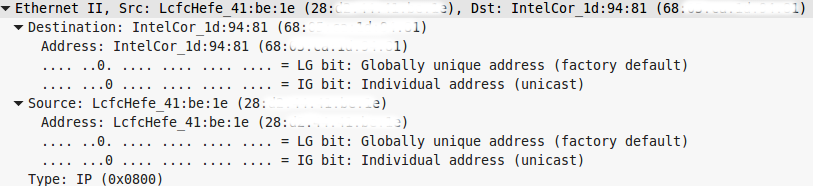
\includegraphics[width=1\linewidth]{images/wireshark-EthernettII.png}
	\caption{Aufbau des Headers in Schicht 2, Auszug aus WireShrak (MAC-Adressen entfernt)}
\end{figure}
Die Frames werden hier dem Ziel, einem Netzwerkteilnehmer, zugestellt, welcher im Header des Frames mit der MAC-Adresse vermerkt ist. Das ist der wesentliche Unterschied zum Hub, welcher die empfangenen Daten an alle Teilnehmer gesendet hat.

Ein Layer-3-Switch oder Multilayerswitch verfügt über mehr Funktionen als ein einfacher Switch. So können zum Beispiel Steuer- und Überwachungsfunktonen genutzt werden, wie IP-Filterung oder Routing. Im Prinzip verletzen diese Funktionalität das ISO-/OSI-Schichtenmodell, allerdings wird die Weiterleitung von Pakete auf der Hardware realisiert, was sehr viel schneller geht als über einen Router.
\\ \\
Der Einsatz eines Switches bringt im Verglich zu den Vorgängern Hub und Bridge einige Vorteile mit sich, hier sei im Besonderen darauf hingewiesen, dass der Switch die Datensicherheit erhöht, denn die Daten werden nur den Netzwerkteilnehmer gesendet, an welchen die Informationen adressiert sind (wenn die MAC-Adresse bekannt ist).

\subsubsection{Funktion der Switch-Tabelle}
Die Switch-Tabelle ermöglicht den wesentlichen Punkt in der Funktionsweise eines Switch: dass die Daten nur noch zu einem bestimmten Empfänger gelangen. \cite[Kapitel 5]{netzwerkeI}
\begin{figure}[H]
	\centering
	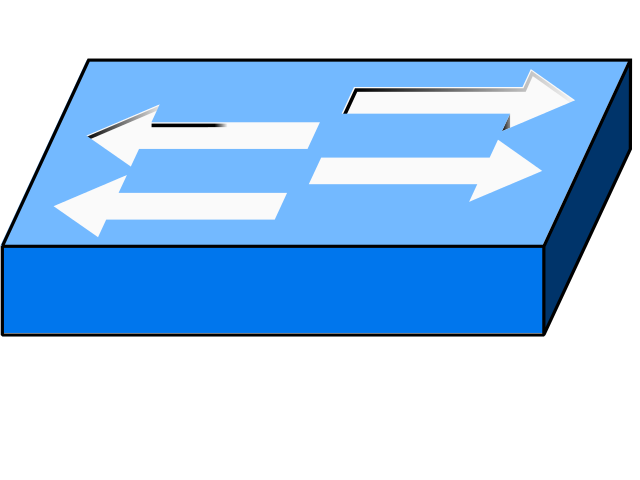
\includegraphics[width=0.3\linewidth]{images/switch.png}
	\caption{Switch \cite{switch-bild}}
\end{figure}
Ein Switch verfügt über Ein- und Ausgänge, die sogenannten Ports. Diese können unabhängig von einander senden und empfangen. Damit keine Frames verloren gehen, verfügt der Switch über einen Datenpuffer.
An den Ein- und Ausgängen sind die einzelnen Netzwerkteilnehmer angeschlossen. In der Switch-Tabelle ist für jeden Port die MAC-Adresse des angeschlossenen Teilnehmers hinterlegt.
\begin{figure}[H]
	\centering
	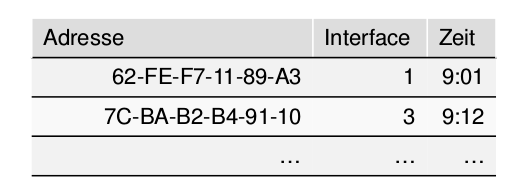
\includegraphics[width=0.7\linewidth]{images/switch-tabelle.png}
	\caption{Switch-Tabelle mit eingetragenen MAC-Adressen und den Ports, hier Interfaces genannt \cite[Kapitel 5, Abbildung Folie 39]{netzwerkeI}}
\end{figure}
Somit kann entschieden werden, an welchen Port der eingegangene Frame gesendet wird.
Es gibt unterschiedliche Arbeitsweisen, nach welchen ein Switch funktioniert. Store-and-Forward wird von jedem Switch umgsetzt, deshalb wird hier auch nur diese betrachtet.

Store-and-Forward ist von den Switch-Methoden die sicherste, allerdings auch die langsamste.
Wird vom Switch ein Frame empfangen, werden die folgenden Schritt bearbeitet.
\begin{enumerate}
\item Schritt
	\begin{itemize}
	\item Switch empfängt gesamtes Frame (store)
	\item berechnet Prüfsumme (CRC)
	\item wenn Prüfsumme nicht mit CRC-Wert im Frame übereinstimmt, wird das Frame verworfen (keine fehlerhaften Daten im lokalen Netzwerk)
	\end{itemize}
\item Schritt
	\begin{itemize}
	\item überprüfen, ob Quell-Adresse in Switch-Tabelle vorhanden ist
	\item wenn nicht, Quell-MAC-Adresse zusammen mit Port in der Tabelle ergänzen
	\item wenn schon vorhanden, lediglich Aging-Timer aktualisieren
	\end{itemize}
\item Schritt
	\begin{itemize}
	\item Zieladresse des Frames mit Eintrag in der Switch-Tabelle vergleichen
	\item ist Zieladresse vorhanden, wird das Frame an den Empfänger weitergeleitet
	\item ist die Zieladresse (noch) nicht vorhanden, wird das Frame an alle Ports weitergeleitet
	\end{itemize}
\end{enumerate}

In einem IPv4-Netzwerk wird der Eintrag in der Switch-Tabelle meist schon von dem ARP-Request (Address Resolution Protocol) mit entsprechendem Port hinterlegt. Dabei wird zunächst aus der ARP-Anfrage der Empfänger herausgelesen und zugeordnet. Ist dieser schon in der Tabelle hinterlegt, brauch da nichts weiter vorgenommen werden. Aus der ARP-Response erhält man folglich den Empfänger, dieser wird in die Switch-Tabelle eingetragen.
Das ARP-Protokoll wird genutzt, um Netzwerkteilnehmer untereinander bekannt zu machen, z.B. Rechner mit Router.
Die Switch-Tabelle füllt sich demnach automatisch und braucht nicht zu konfiguriert zu werden.

\subsubsection{Was passiert, wenn die Switch-Tabelle überläuft}
Ist die Tabelle gefüllt mit Einträgen und kann keinen neuen Eintrag mehr aufnehmen (die Tabelle könnte zu klein sein), werden alle Frames, die nicht zugeordnet werden können, an alle Ports gesendet werden. Das würde die Netzwerklast drastisch heben.